\documentclass{article}

\usepackage{graphicx}
\usepackage{tikz}
\usepackage{tikzsymbols}
\usetikzlibrary{calc,patterns,shapes.geometric}
\pagestyle{empty}
\usepackage[margin=0pt]{geometry}
\geometry{papersize={14in,12in}}

\def\centerarc[#1](#2)(#3:#4:#5){\draw[#1] ($(#2)+({#5*cos(#3)},{#5*sin(#3)})$) arc (#3:#4:#5);}

\begin{document}
	\begin{figure}
		\centering
		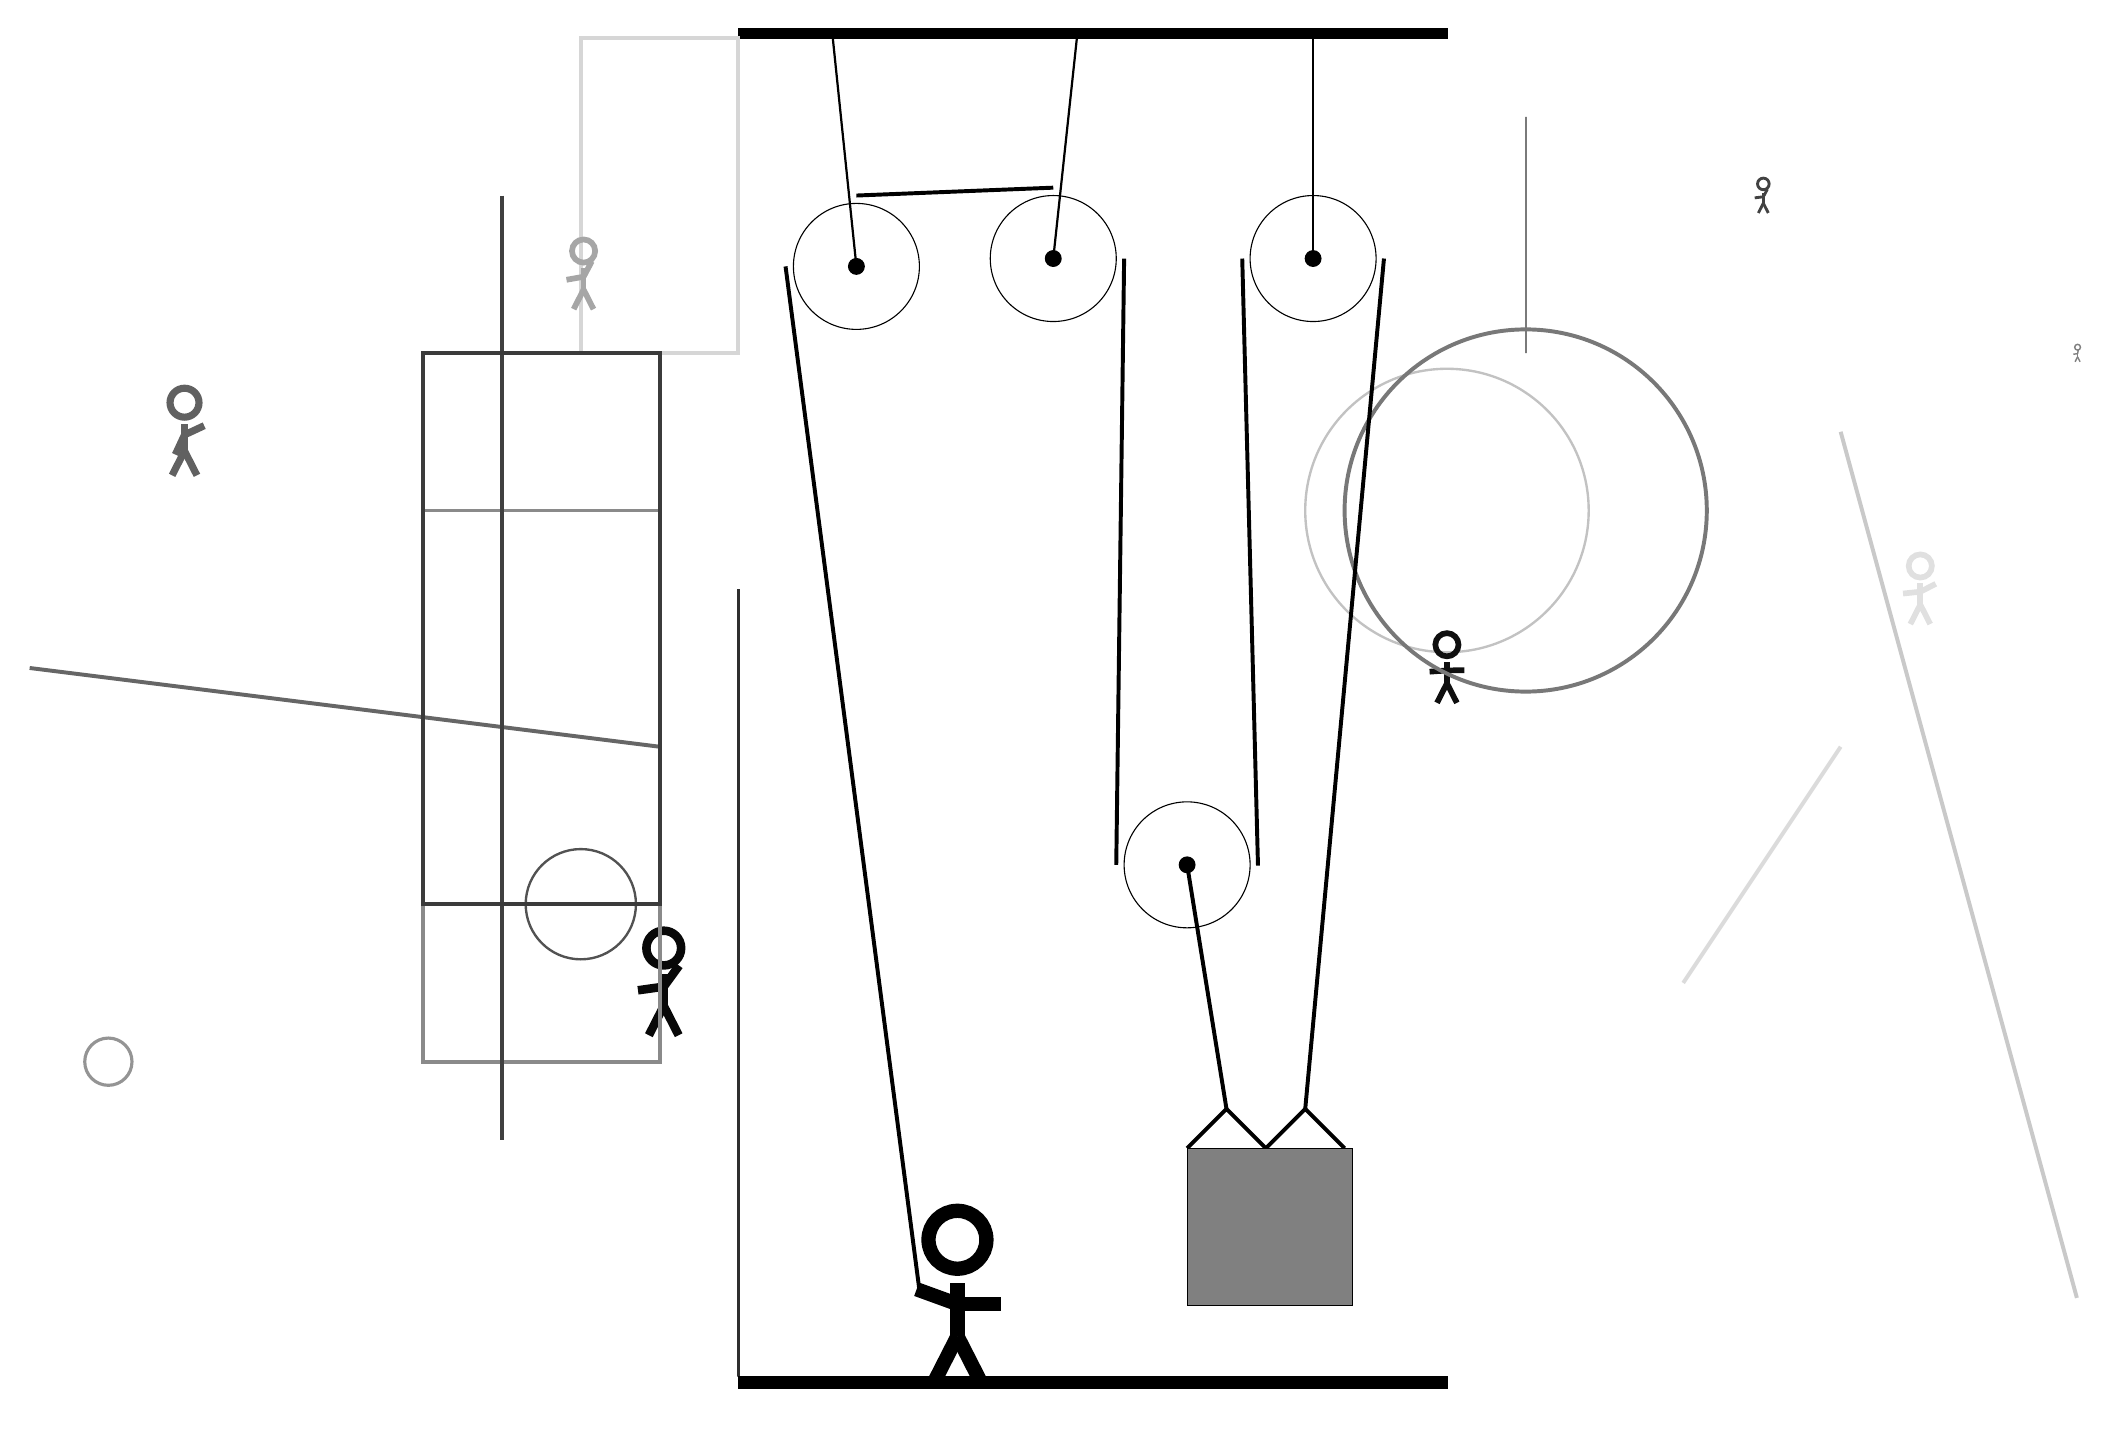
\begin{tikzpicture}
			%%%%% START %%%%%
			
			\draw[fill=black] (-3, 14) rectangle (6, 14.125);
			
			\draw (1, 11.2) circle (0.8);
			\draw[fill=black] (1, 11.2) circle (0.1);
			\draw[thick] (1, 11.2) -- (1.3, 14);
			
			\draw (4.3, 11.2) circle (0.8);
			\draw[fill=black] (4.3, 11.2) circle (0.1);
			\draw[thick] (4.3, 11.2) -- (4.3, 14);
			
			\node[line width=0.6mm, color=black!97] at (-4, 2) {\Strichmaxerl[6][8][54]};
			
			\draw[line width=0.5mm, color=black!60](-4, 5) -- (-12, 6);
			\draw [line width=0.3mm, color=black!68](-5, 3) circle (0.7);
			\draw [line width=0.3mm, color=black!24](6, 8) circle (1.8);
			\draw[line width=0.2mm, color=black!52] (7, 13) rectangle (7, 10);
			\node[line width=0.5mm, color=black!74] at (10, 12) {\Strichmaxerl[2][7][62]};
			\draw [line width=0.3mm, color=black!94](-11, 2) circle (0.0);
			\draw[line width=0.4mm, color=black!82] (-3, -3) rectangle (-3, 7);
			\node[line width=0.6mm, color=black!12] at (12, 7) {\Strichmaxerl[4][6][27]};
			\draw[line width=0.5mm, color=black!16] (-3, 10) rectangle (-5, 14);
			
			\draw[line width=0.5mm, color=black!46] (-4, 1) rectangle (-7, 8);
			\draw[line width=0.5mm, color=black!14](9, 2) -- (11, 5);
			\draw[line width=0.5mm, color=black!21](11, 9) -- (14, -2);
			\node[line width=0.4mm, color=black!62] at (-10, 9) {\Strichmaxerl[5][65][25]};
			\draw[line width=0.5mm, color=black!75](-6, 12) -- (-6, 0);
			\node[line width=0.7mm, color=black!35] at (-5, 11) {\Strichmaxerl[4][10][62]};
			
			\draw[line width=0.5mm, color=black!77] (-4, 3) rectangle (-7, 10);
			
			\draw [line width=0.4mm, color=black!42](-11, 1) circle (0.3);
			\node[line width=0.7mm, color=black!94] at (6, 6) {\Strichmaxerl[4][4][1]};
			\draw [line width=0.5mm, color=black!53](7, 8) circle (2.3);
			\node[line width=0.3mm, color=black!50] at (14, 10) {\Strichmaxerl[1][8][79]};
			
			
			\draw (2.7, 3.5) circle (0.8);
			\draw[fill=black] (2.7, 3.5) circle (0.1);
			
			\draw[line width=0.5mm]  (2.7, -0.1) -- (3.2, 0.4) -- (3.7, -0.1) -- (4.2, 0.4) -- (4.7, -0.1);
			\draw[fill=black!50] (2.7, -0.1) rectangle (4.8, -2.1);
			
			\draw (-1.5, 11.1) circle (0.8);
			\draw[fill=black] (-1.5, 11.1) circle (0.1);
			\draw[thick] (-1.5, 11.1) -- (-1.8, 14);
			
			\draw[line width=0.5mm](-0.7, -1.9) --  (-2.4, 11.1);
			\centerarc[line width=0.5mm](-1.5, 11.1)(90:180:0.9);
			\draw[line width=0.5mm](-1.5, 12.0) -- (1, 12.1);
			\centerarc[line width=0.5mm](1, 11.2)(0:90:0.9);
			\draw[line width=0.5mm](1.9, 11.2) -- (1.8, 3.5);
			\centerarc[line width=0.5mm](2.7, 3.5)(180:370:0.9);
			\draw[line width=0.5mm] (3.6, 3.49) -- (3.4, 11.2);
			\centerarc[line width=0.5mm](4.3, 11.2)(0:180:0.9);
			\draw[line width=0.5mm](4.2, 0.4) -- (5.2, 11.2);
			\draw[line width=0.5mm] (3.2, 0.4) -- (2.7, 3.5);
			
			\node at (-0.2, -2) {\Strichmaxerl[10][-20][0]};
			
			\draw[fill=black] (-3, -3) rectangle (6, -3.15);
			
			%%%%% END %%%%%
		\end{tikzpicture}
	\end{figure}	
\end{document}